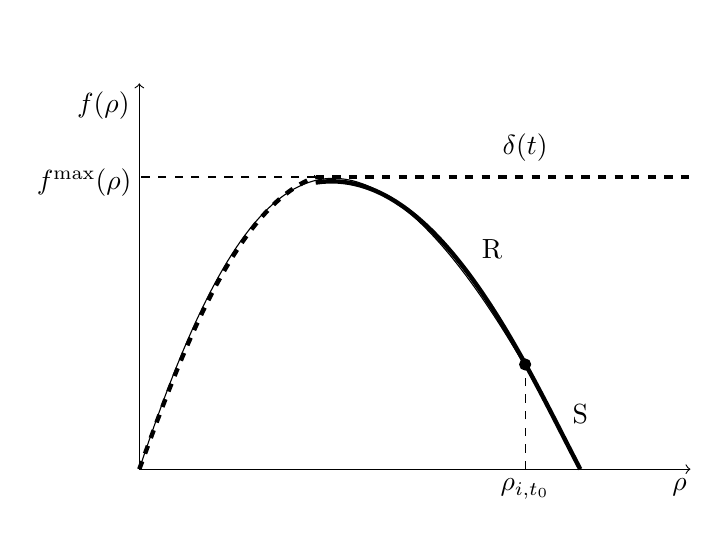
\begin{tikzpicture}[scale=1.4]
\draw [<->](0,3.5)--(0,0) -- (5,0);
\draw (0,0) .. controls (1,3) and (2,4) .. (4,0);
%\draw[fill=black](0.73,1.8) circle (0.05);
\draw[ultra thick](4,0)..controls (3.5,0.95) and (2.7,2.77) .. (1.6,2.6);
\draw[fill=black](3.5,0.95) circle (0.05);
\draw[ultra thick, dashed](0,0)..controls (0.35,0.95) and (0.85,2.38) .. (1.6,2.65);
\draw[ultra thick, dashed] (1.6,2.65) -- (5,2.65);
\draw[dashed] (1.6,2.65) -- (0,2.65);
%\draw (0,0) .. controls (1,3) and (2.5,1) .. (3,0);
%\draw (0,1)--(2.5,2.28);
%\draw (0,0) -- (1,0.52)--(3.08,1.6);
%\draw [ ultra thick, red] (0.73,1.8)--(3.5,0.95);
%\draw [dashed] (0.73,0)--(0.73,1.8); 
%\draw [dashed] (0.73,1.8)--(2.9,1.8);
\node (above) at (3.2,2) {R};
\node (above) at (4,0.5) {S};
\draw [dashed] (3.5,0)--(3.5,0.95);
\node [below] at (4.9,0) {$\rho$};
\node [left] at (0,3.3) {$f(\rho)$};
%\node [below] at (3.1,0.08) {$\rho^*$};
\node [below] at (3.5,0.0) {$\rho_{i,t_{0}}$};
\node [above] at (3.5,2.7) {$\delta(t)$};
\node (left) at (-0.5,2.6) {$f^{\max}(\rho)$};
%\node [below] at (0.73,0) {$\rho_{i,0}$};
%\node [above] at (1.5,1.71) {$V_b$};
\end{tikzpicture}